\subsection{A deblending test}
\label{sec:deblending_test}

We demonstrate the performance of StarNet on deblending two stars. Two stars were simulated in an $7\times 7$ image with two bands. 
The input to StarNet was the entire $7\times 7$ image; no tiling was used in this experiment. 
We fitted StarNet using the sleep phase, with prior described in Section~\ref{sec:gen_model}, except that the number of stars was uniform: with equal probability, there is either 0, 1, or 2 stars in the image. 

Figure~\ref{fig:deblending_fig} displays the probability that $N = 2$ under the fitted variational posterior, as the distance between two stars varies.
As expected, the probability of $N=2$ increases as the separation increases. 
In addition, the stars become easier to deblend as the flux increases (Figure~\ref{fig:deblending_fig}a).
In Figure~\ref{fig:deblending_fig}b, the flux of the first star was set at 4000nelec, and the flux of the second star was varied. 
As the difference in flux between the two stars increases, the stars become harder to deblend. 
Finally, in Figure~\ref{fig:deblending_fig}c, the flux of the first star was set at 4000nelec in both bands. The second star had flux 4000nelec in the first band, and its flux in the second was varied. 
This demonstrates the benefits of multiband deblending: color, 
the relative fluxes in neighboring bands, aids in differentiating stars. 

\begin{figure}[!h]
    \centering
    \begin{subfigure}{0.95\textwidth}
        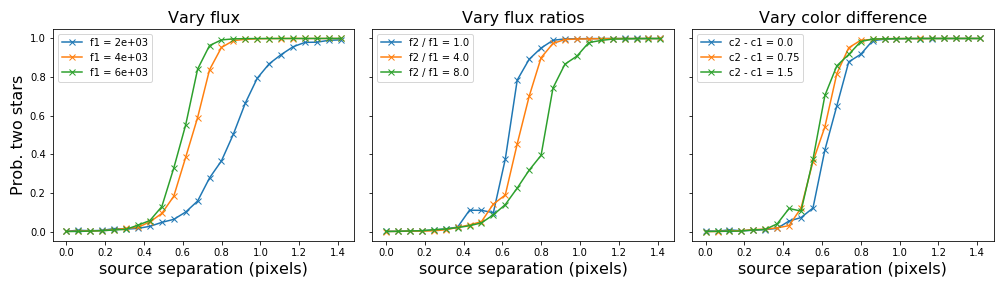
\includegraphics[width=\textwidth]{figures/deblending_test.png}
    \end{subfigure}
      \begin{subfigure}{0.95\textwidth}
        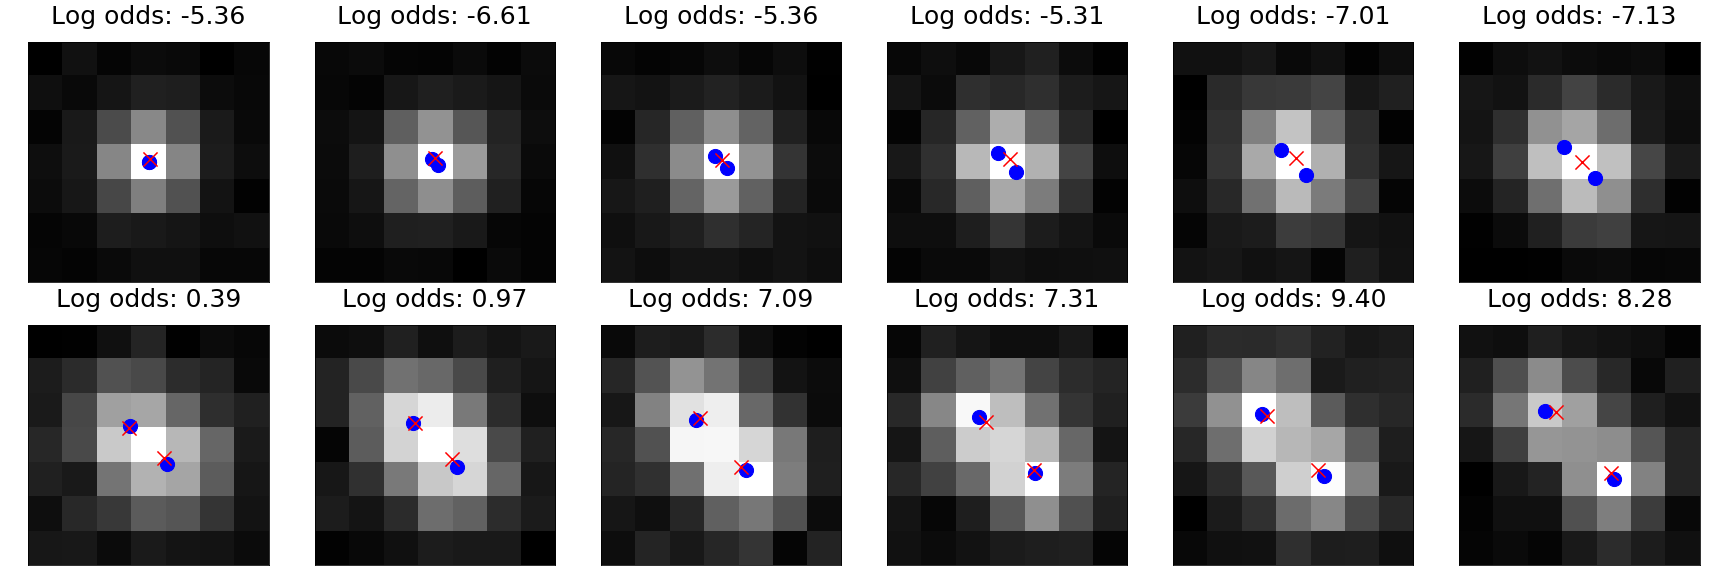
\includegraphics[width=\textwidth]{figures/deblending_ex.png}
    \end{subfigure}
    \caption{(Top row) The probability under $q$ that the image region contains two stars as source separation increases.
    (Bottom) An example of StarNet detections as source separation increases. Red are estimated locations, defined by the the mode of the variational distribution; blue are true locations. Log odds are probability of two stars over probability of one star. Here, both stars have a flux of 4000nelec.}
    \label{fig:deblending_fig}
\end{figure}
